%
% Documentation of the planar geometry algorithms used in the
% Mini Jam project du on October 31st, 2024.
%
% Compute the intersections of a straight line with an ellipse and
% a rectangle.
%
\documentclass[11pt]{article}
%
% Packages
%
\usepackage{graphicx}
% \usepackage{algorithmic}
\usepackage{amsmath}
%
% Definitions
%
% \newcommand{\sign}{\hbox{sign}}
%
% Dimensions
% \setlength{\textwidth}{5.5in}
% \setlength{\textheight}{8.4in}
% \setlength{\hoffset}{-0.25in}
% \setlength{\topmargin}{0pt}
\setlength{\parindent}{0pt}
% \setlength{\parskip}{0.5\baselineskip}
%
% Definitions
\newcommand{\Rb}{{\bf{R}}}
\newcommand{\eqn}[1]{(\ref{#1})}
\newcommand{\TODO}{{\bf TODO}}
\newcommand{\bhat}{{\hat b}}
\newcommand{\xhat}{{\hat x}}
\newcommand{\yhat}{{\hat y}}

\begin{document}
%
%
\title{Planar Geometry}
\author{Aurel Wisse}
\maketitle
%
%
\begin{abstract}
Documentation of the planar geometry algorithms used in the
Mini Jam project due on October 31st, 2024. We present the algorithms used to
compute the intersection of straight lines (sensor capture of obstacles) with
circles and convex polygons.
\end{abstract}

%
\section{Straight Line}
\label{sec:straight:line}

Representation of a straight line going through
coordinates $(x_0, y_0)$ and $(x_1, y_1)$. Determine the points $(x, y)$ on the
line.

We have two special cases: 
\begin{eqnarray}
    (x, y) &=& (x_0, y)\quad\forall y\in\Rb\quad \text{ if } x_1 = x_0 \\
    (x, y) &=& (x, y_0)\quad\forall x\in\Rb\quad \text{ if } y_1 = y_0
\end{eqnarray}

For the general case, $x_0 \neq x_1, y_0 \neq y_1$, we have
\begin{eqnarray}
    y &=& ax+b,\quad \text{where} \label{eq:line:general}\\
    a &=& \frac{y_0 - y_1}{x_0 - x_1}, \notag \\
    b &=& \frac{x_0 y_1 - y_0 x_1}{x_0 - x_1} \notag
\end{eqnarray}

\subsection{Line Segment}
\label{sec:line:segment}

For the special case $x_0 = x_1$ a line segment $[(x_0, y_0):(x_0, y_1)]$ 
between $(x_0, y_0)$ and $(x_0, y_1)$ is given by the equation
\begin{equation}
    (x, y) = (x_0, y)\quad y\in [y_0, y_1]
\end{equation}

For the special case $y_0 = y_1$ a line segment $[(x_0, y_0):(x_1, y_0)]$ 
between $(x_0, y_0)$ and $(x_1, y_0)$ is given by the equation
\begin{equation}
    (x, y) = (x, y_0)\quad x\in [x_0, x_1]
\end{equation}

For the general case given by \eqn{eq:line:general}, the line segment 
\begin{gather*}
    \left[(x_0, y_0):(x_1, y_1)\right]
\end{gather*}
between $(x_0, y_0)$ and $(x_1, y_1)$ is given by
\begin{equation}
    (x, y) = (x, ax + b)\quad x\in [x_0, x_1]
\end{equation}

\section{Polygons}
\label{sec:polygons}

We are concerned with a general polygon in the two-dimensional plane. A polygon
with $n$ sides is well defined by $n$ line segments and $n$ points $(x_0,
y_0),\ldots,(x_{n-1}, y_{n-1})$. The $n$ sides are defined by the line segments
\begin{equation}
    \left\{[(x_i, y_i):(x_{i+1}, y_{i+1})], i=0,\ldots,n-2\right\}\\
\cup\left\{[(x_{n-1}, y_{n-1}):(x_{0}, y_{0})]\right\}
\end{equation}

\section{Circle}
\label{sec:circle}

The standard implicit equation for a circle of radius $r$  centered at the 
point $(x_0, y_0)$ is
\begin{equation}
    (x - x_0)^2 + (y - y_0)^2 = r^2 
\end{equation}

\TODO: We might generalize to an ellipsis later:
\begin{equation}
    \frac{(x-x_0)^2}{a^2} + \frac{(y-y_0)^2}{b^2} = 1
\end{equation}

\section{Intersection}
\label{sec:intersection}

\subsection{Line Segment}
\label{sec:intersection:line:segment}
The intersection of a straight line $y=ax+b$ (a sensor ray) with a line segment
$y = a_s x + b_s, x\in[x_0, x_1]$ is given by 
\begin{equation}
    ax+b = a_sx+b \land x_0 < x < x_1
\end{equation}

\subsection{Circle}
\label{sec:intersection:circle}
The intersection of a straight line $y=ax+b$ with a circle 
$(x-x_0)^2+(y-y_0)^2=r^2$ is given by
\begin{equation}
    (x-x_0)^2 + (ax+b - y_0)^2 = r^2 
\end{equation}
In order to simplify calculations, we translate the origin to $(x_0, y_0)$. Let
\begin{equation}
    \xhat = x-x_0,\quad \yhat = y-y_0,\quad \bhat = ax_0 + b - y_0.
\end{equation}
The intersection of the straight line $\yhat = a\xhat + \bhat$ with the circle
$\xhat^2 + \yhat^2 = r^2$ is given by
\begin{equation}
    \xhat^2 + (a\xhat + \bhat)^2 = r^2 \label{eq:intersection:circle}
\end{equation}
The solutions $\xhat$ to \eqref{eq:intersection:circle} are given by
\begin{equation}
    \xhat = -\frac{a\bhat}{1+a^2}\pm 
        \sqrt{\frac{1}{1+a^2}\left(r^2-\bhat+\frac{a^2 b^2}{1+a^2}\right)}
\end{equation}
From this, we see that if 
\begin{equation}
    \frac{1}{1+a^2}\left(r^2-\bhat+\frac{a^2 b^2}{1+a^2}\right) < 0, \notag
\end{equation}
there is no intersection of the line and the circle.

\section{Representation}
\label{sec:representation}
In this section we describe how circles, sensor rays and line segments will be
represented in code. There is no particular polygon object given that a
polygon is just a collection of line segments.

\subsection*{Straight line}

Parameters $a, b, X$. 

\begin{enumerate}
    \item For a  straight horizontal line, $a=X=0, y=b$.
    \item For a  straight vertical line, $a=b=0, x=X$.
    \item For a general line, $X=0$.
\end{enumerate}

\subsection*{Line Segment}

Parameters $x_0, y_0, x_1, y_1$. 

Covers all cases. We must define a transformation of the parameters into a
general straight line with inequalities:
\begin{eqnarray*}
    (a, b, X) = (0, y_0, 0) ,\, x_0 < x < x_1 &\text{if}& 
        y_0 = y_1\\
    (a, b, X) = (0, 0, x_0) ,\, y_0 < y < y_1 &\text{if}& 
        x_0 = x_1\\
    (a, b, X) = \left(\frac{y_0 - y_1}{x_0-x_1},
            \frac{x_0 y_1 - x_1 y_0}{x_0 - x_1}, 0\right),\,
    x\in[x_0, x_1] &\text{if}& x_0\neq x_1 \land y_0\neq y_1
\end{eqnarray*}

\subsection*{Circle}

Parameters $x_0, y_0, r$.

\section{Game Objects}
\label{sec:game:objects}
There are four types of objects in the game. 
\begin{enumerate}
    \item The game surface. A rectangle with $(0,0)$ in the upper left corner. 
        It is defined by two values $x_G > 0, y_G>0$ respectively on the x-axis
        and the y-axis.
    \item The {\sl vehicle} which is a rectangle, a collection of four line
        segments.
    \item The target which is a single point $T = (x_T, y_T)$ on the game
        surface.
    \item The obstacles. A collection of line segments and circles.
\end{enumerate}

\section{The Game}
\label{sec:the:game}
\begin{itemize}
    \item There are two players in the game, one on each Arduboy. 
    \item The objective of the game is to reach the target first without 
        running into an obstacle. 
    \item Running into an obstacle requires a repair of the vehicle and leads 
        to a 30 second suspension. 
    \item Colliding with the other players car from the side or behind places
        the player at the start with a 30 second suspension.
    \item A frontal collision of both players ends the game without a winner.
\end{itemize}

\section{User Interface}
The main screen 
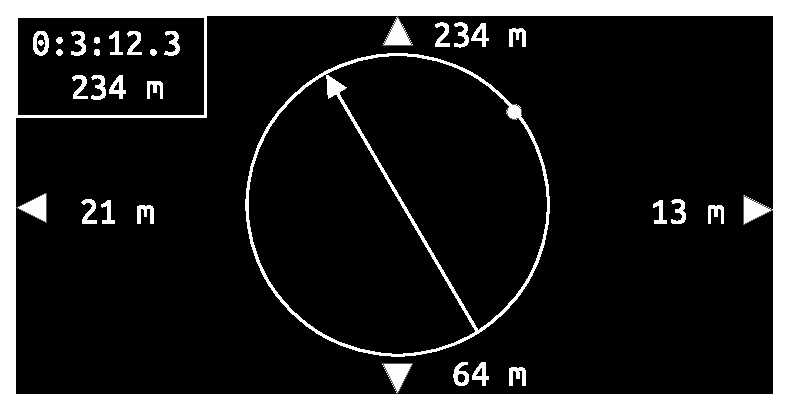
\includegraphics{screen.eps}

\section{Scanning}
\label{sec:scanning}

In each frame, the vehicle scans for obstacles in the following way.

In this section, we define how the car scans continuously 
\end{document}
